\documentclass[a4paper,twoside]{article}

\usepackage{epsfig}
\usepackage{subfigure}
%\usepackage{stfloats}
\usepackage{algorithm}
\usepackage{algorithmic}	
\usepackage{calc}
\usepackage{amssymb}
\usepackage{amstext}
\usepackage{amsmath}
\usepackage{amsthm}
\usepackage{multicol}
\usepackage{pslatex}
\usepackage{apalike}
\usepackage{SciTePress}
\usepackage[small]{caption}
\usepackage{eqparbox}
\renewcommand{\algorithmiccomment}[1]{\hfill\eqparbox{COMMENT}{\# #1}}

\subfigtopskip=0pt
\subfigcapskip=0pt
\subfigbottomskip=0pt

\begin{document}

%ZJW: this is a slightly ambitious title, but it is a start
\title{Reconstruction of Fine Level Geometric Structure From Stereo Pairs in the Underwater Setting}

\author{\authorname{Timothy M. Peters*, Erik A. Nelson*, Tyler Vitti, Timothy Gambin, \\Christopher M. Clark, and Zo\"{e} J. Wood}
\affiliation{California Polytechnic State University, San Luis Obispo, CA, U.S.A.}
\thanks{(Author)* denotes equal contributions }
\thanks{This material is based upon work supported by the National Science Foundation under Grant No. 0966608.}%
}

\keywords{3D Site Reconstruction: Surface Reconstruction: Underwater Stereo Vision: Projective Texturing}

\abstract{The study of underwater structures, such as wells, cisterns, and water storage systems, can be of historical and scientific significance for archeologists. However, access to and study of such sites can be dangerous or infeasible for humans.
Underwater micro-ROVs, such as the VideoRay Pro III GTO, can often reach and navigate these locations more safely while causing less harm to the site.
Prior work has successfully reconstructed geometric models of such underwater structures with the use of sonar measurements. Although effective, sonar has a limited resolution and omits many fine geometric details of the model in the scanning process. In this paper, we present a preliminary solution towards the accurate reconstruction of fine details of geometric features in the underwater setting using stereo pairs. These fine details can then integrated into 3D models reconstructed from sonar to create a more accurate final model of a water system. The initial rough 3D model is generated using multiple sonar scans of the walls of the site. The fine details of the internal organic surfaces are recorded using stereoscopic imaging. Finally, the rough 3D model is deformed and textured using the details obtained through stereoscopic imaging. 
We present initial results and detailed methodology for future data acquisition.
}

\onecolumn \maketitle \normalsize \vfill

\section{\uppercase{Introduction}}
\label{sec:introduction}

%Related works and an overview of the procedure. Possibly system block diagram leading the reader through the process.
%ZJW, yes we need a system block diagram - can you make one Erik? Tim?

\noindent Recent research in the field of mobile robotics has demonstrated the creation of 3D maps of settings otherwise inaccessible to humans, such as narrow tunnels and difficult to navigate marine caves~\cite{ICEX11,McVicker,McVicker2}. Progress made in Simultaneous Localization and Mapping (SLAM) algorithms  (\cite{Williams2000}, ~\cite{harbor}, and \cite{Fairfield2005,Fairfield2006}) allow robots to localize themselves and create these maps using input from sonar, infrared, and other scanning sensors. Such maps, or evidence grids, can then be treated as implicit volumes to construct a geometric model of the scanned regions using marching cubes~\cite{Lorensen}. An example of a geometric model of a well used for water storage, can be seen in Figure~\ref{fig:}.
Unfortunately, due equipment limitations, sensor noise, and probabilistic uncertainty occurring in the  data acquisition process, these models often suffer from a loss of fine geometric details. Loss of detail in the scanning process is a problem for end-users, who wish to study these models or use them for educational purposes.
 %We examine a case in which a sonar sensor is used to extract surface data in an underwater environment.
%Error is furthered in this case by equipment drift during scans and floating occlusions, both of which lead to geometric misrepresentations.
In this paper we present a preliminary solution towards the reintroduction of fine details omitted by sonar data into surface reconstructions.  
Two cameras are used to capture stereo images of underwater surfaces.
The stereo images are then processed to produce disparity maps which contain the fine geometric detail of the original surface.
Each disparity map can then be used to enhance the final geometric model.

This project is a part of a larger ongoing project, with the broad goal of mapping and modeling ancient water storage systems, i.e. cisterns, wells and water galleries located in most houses, churches, and fortresses of the islands of Malta, Gozo, and Sicily. This multiple year project involves the deployment of a micro-ROV into water systems in the Mediterranean~\cite{White10,ICEX11,McVicker,McVicker2} with this paper documenting the first use of stereo data for fine level geometry acquisition. The data used in this paper was gathered through a series of underwater robot deployments in which multiple sonar scans were gathered, then fused into a map of the scene via Simultaneous Localization and Mapping (SLAM) algorithms. In addition to the sonar data, stereo pairs were obtained for use in creating disparity maps to model fine level geometry. In order incorporate the disparity information with the general surfaces, both the color data and disparity information is projectively textured onto the pre-established gross sonar generated 3D model. Finally, the geometry contained within the frustums of the projectors in the model is displaced in accordance with the projected disparity maps, preserving the fine details omitted in earlier stages of reconstruction. The stages of our algorithm can be seen in Figure~\ref{fig:systemBlock}.

%The accurate surface reconstruction solution proposed in this paper involves four steps. First, an occupancy grid of the acquired sonar data is generated by mosaicing sonar scans together with a simultaneous localization and mapping (SLAM) algorithm. Next, a hole filling algorithm is used to probabilistically complete the occupancy grid and form a closed surface, which is extrapolated into 3D and stored as a mesh. Meanwhile, disparity maps are created from stereo image pairs captured on the HD cameras in multiple locations. Finally, a projective texturing and depth extraction algorithm is used to project the generated disparity maps from multiple locations onto surfaces of the mesh, and subsequently displace the vertices intersecting the projector's view frustum according to the disparity map's color values. 

The results reported in this paper are from preliminary work in a multidisciplinary setting, utilizing aspects of emerging robotics and computer graphics technology.  This paper outlines the data acquisition and stereo displacement map computation, describes our preliminary novel solution to displacing rough geometry in accordance with a projected disparity map, illustrates our results on a partial model using existing data, and outlines a data acquisition process for future missions. The goal of this work is the generation of a computer model which includes the fine organic features found in underwater storage systems.

\begin{figure*}[!ht]
  \vspace{-0.2cm}
  \centering{
     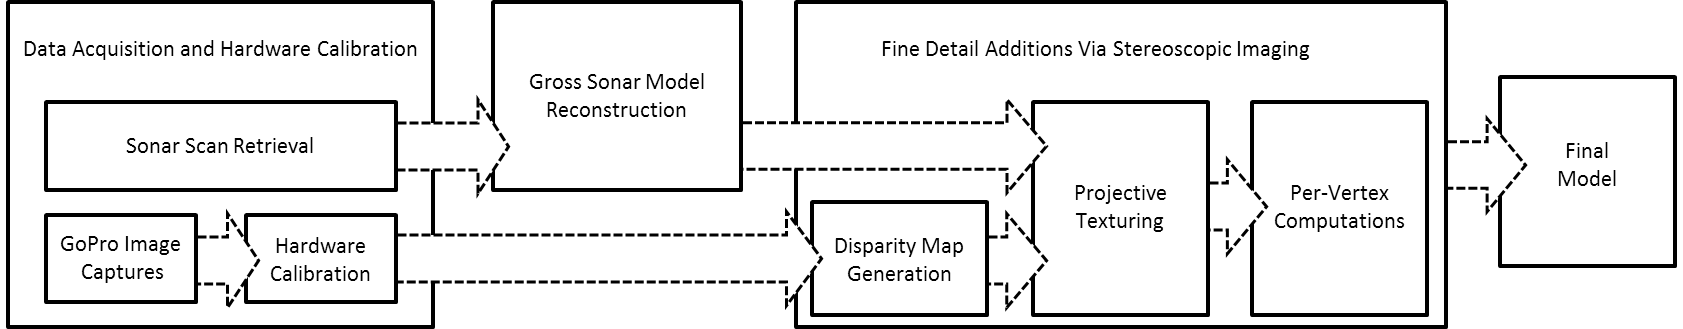
\epsfig{file = pics/systemBlock.png, width = \textwidth}}
  \caption{Pipeline for fine detail additions to sonar generated meshes.}
 \label{fig:systemblock}
\end{figure*}

\section{\uppercase{Related Work}}
\label{sec:data}

This project relies on data acquired from algorithms for mapping with underwater robots (e.g. \cite{Williams2000}, ~\cite{Williams09}, ~\cite{opizarro-2009a}, \cite{Fairfield2005,Fairfield2006}, \cite{Clark2008b}, and~\cite{White10}). For a good survey of the core techniques capable of fusing data from multiple sensors, see Thurn~\cite{Thrun2005}.
For this project the most relevant  research in underwater robot Simultaneous Localization and Mapping (SLAM) is found in (e.g. \cite{Williams2000}, ~\cite{harbor}, and \cite{Fairfield2005,Fairfield2006}).  

In addition, this work relies on well known algorithms from computer graphics, such as surface extraction from volume data using marching cubes~\cite{Lorensen}, projective texturing and texture mapping~\cite{Williams78castingcurved,Segal} and the use of vertex shaders to displace existing vertices on the GPU. Work in ~\cite{Fairfield:2010} likewise uses marching cubes to create a geometric model of underwater structures from an evidence grid, but uses a much more complex ROV and sensors

This work also relies on related work in the field of stereoscopic data acquisition and disparity map reconstruction~\cite{stereo:gutMarroquin},~\cite{stereo:scharsteinSzeliski}.
  In particular, this work uses the method of~\cite{stereo:zitKan}.
  The work of~\cite{stereo:nalGast} was also consulted to compensate for differences in light intensities between images.
  This paper explores the conversion of images into the HSL color space in an attempt to remove light intensity from the equation and compare solely at hue and saturation values.
  Unfortunately, the underwater setting does not transmit colors well, forcing the use of more common stereo-vision comparisons~\cite{stereo:nalpantidis2008review}. 

\section{\uppercase{Data Acquisition and Hardware Calibration}}
\label{sec:data}

\noindent The goal of this project is to acquire geometric models of underwater structures found in the Mediterranean.  We describe the exact hardware and data acquisition process used in this project.
%Discuss the hardware mounted onto the ROV, and the process by which we collected data

A micro submersible Remotely Operated Vehicle (ROV), specifically a VideoRay Pro III GTO, is utilized in the data acquisition process as a means of navigating cisterns and properly orienting the data collection hardware (Figure~\ref{fig:ROV}). The ROV is deployed into a cistern and guided from a control module above the surface. During deployment, the navigator repeatedly rests the ROV on the cistern floor and records a $360^{\circ}$ stationary sonar scan, then lifts the ROV and repositions it elsewhere in the cistern for another scan until data for the entire horizontal scan plane has been collected. The sonar scans must have some overlap to facilitate mosaicing and localization for surface reconstruction, which is taken into consideration when positioning the ROV on the cistern floor. A complete overview of the sonar data acquisition process can be found in~\cite{ClarkVast}.  This collection of scan planes is then used to build a general 3D model of the cistern in question~\cite{ICEX11}.
  
\begin{figure}[!h]
   \vspace{-0.2cm}
   \centering{
      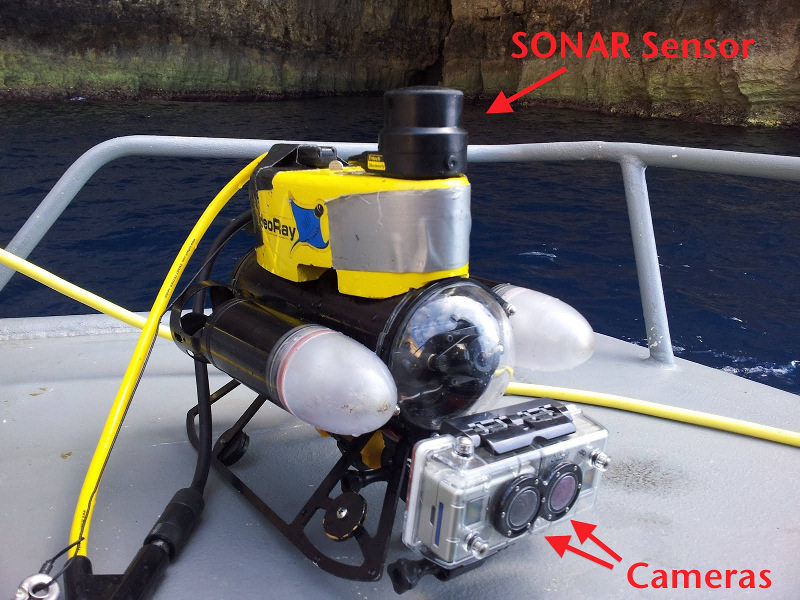
\epsfig{file = pics/ROV.jpg, width = 7cm}}
   \caption{Hardware setup, consisting of a Tritech SeaSprite sonar sensor and two vertically aligned HD GoPro cameras mounted on a VideoRay Pro III GTO micro ROV.}
  \label{fig:ROV}
 \end{figure}

While the ROV is navigating a cistern, two high-definition (HD) cameras mounted to the bow in a waterproof casing are triggered to capture images every \textbf{HOW MANY SECONDS?}. At specific intervals along the cistern wall, the ROV is heldp stationary to take multiple images.
For the images captured in this manner, approximate position and heading of the ROV are recorded and used later to align projectors in the cistern model created through sonar measurements. Corresponding images captured by the pair of stereo cameras are then used to build disparity maps of the features in the cistern, as described below.

%ZJW - Please add more details about the actual mounting and set up - which cameras were used, what underwater housing, how mounted, etc!!!

%Erik - Tim?

\subsection{Hardware Calibration}
To facilitate the accurate virtual reconstruction of the world it was necessary to calibrate the GoPro cameras.
Both the aspect ratio and the vertical field of view (VFOV) needed to be calculated to accurately re-project the captured images and disparity maps in the virtual world.  
The following equations were used:

\begin{align}
\text{Aspect Ratio} &= \frac{\text{width}}{\text{height}} \\
\text{VFOV} &= 2 * tan^{-1}(\frac{\text{height}/2}{\text{depth}})
\end{align}

%\begin{figure}[!h]
%   \vspace{-0.2cm}
%   \centering{
%      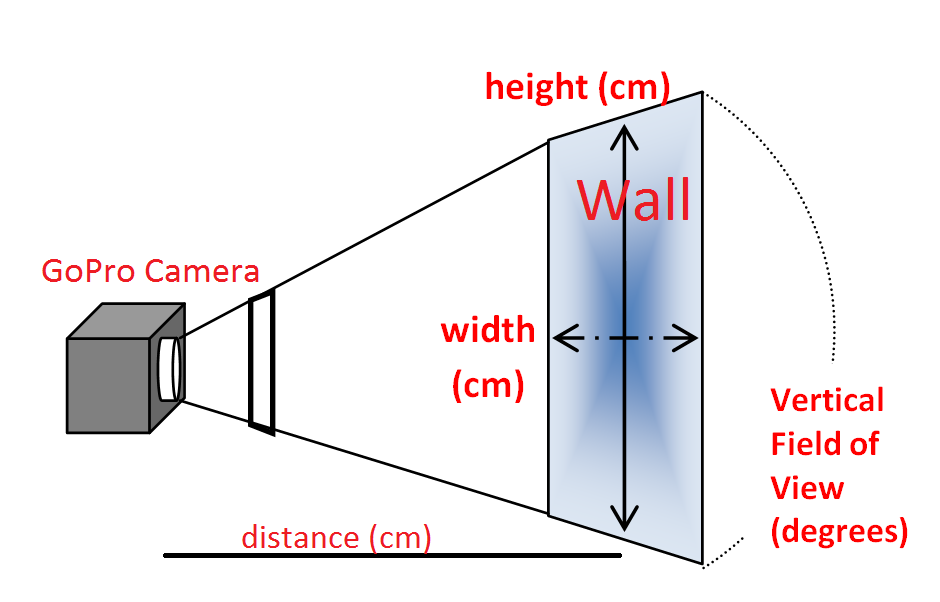
\epsfig{file = pics/CalibrationDimentions.png, width = 7cm}}
%   \caption{GoPro Calibration Measurements}
%  \label{fig:ROV}
% \end{figure}

These two values were used to specify the behavior of projectors, discussed later in Section~\ref{subsec:projectiveTexturing}.

%ZJW: Note this section should be minimal unless you want to put Billy and Jeff on the paper - we more need to treat this as - we get input, which is the gross model
\subsection{{Gross sonar Model Reconstruction}}
\label{sec:reconstruction}

\begin{figure*}[ht!]
   \vspace{-0.2cm}
   \centering{
      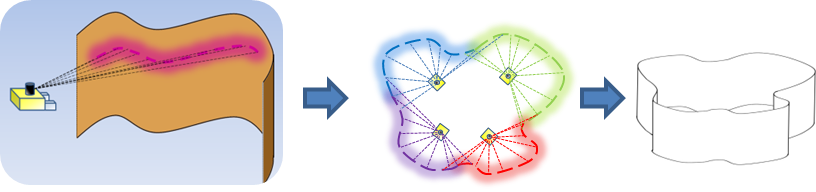
\epsfig{file = pics/1.png, width = 0.9\textwidth}}
   \caption{How we generate meshes from sonar models.}
  \label{fig:meshgen}
 \end{figure*}
 
\noindent This work is focused on reconstructing geometric models from evidence maps representing Mediterranean water storage systems (cisterns, wells and water galleries).  As a pre-process to the algorithms presented here for fine level geometry modeling, the cisterns are mapped using sonar data, which is fused into a two dimensional grid of cells with given a likelihood $p_{i,j} \in [0,1]$ of being occupied \cite{Thrun2005} and~\cite{White10}. This single 2D layer can then be extruded into a 3D evidence grid and be treated as volume data.  A polygonal geometric model of the scanned data can be constructed via marching cubes, where any cell with $p_{i,j}$ greater than a threshold value, $t$, is considered an occupied cell and associated with a wall in the model. $t$ is used to define occupancy and is generally set to values in the range $.65-.85$. We refer the reader to~\cite{ICEX11,McVicker,McVicker2} for more details on the mapping process. See Figure~\ref{fig:meshgen} for an illustration of the general process used to acquire data and generate a geometric model.

%Discuss sonar models/how they are generated in our situation. More focused on the robotics aspect, rather than the details of Jeff and Billy's projects.
%Mention that we extrapolate the near-ground scan plane into 3D in most cases, rather than having true 3D maps.

%\section{\uppercase{Fine Detail Additions Via Stereoscopic Depth Extraction}}
\section{\uppercase{Constructing a more accurate geometric model}}
\label{sec:detail}

\noindent The models constructed from the evidence give a good representation of the gross shape of an underwater system. However, due to challenges in the acquisition process for sonar data, these models tend to lose the fine geometric details present in many of the mapped structures, which are important to archaeologists seeking to study the underwater system. See Figure~\ref{fig:wellNoFine} for an example of a well model constructed from sonar data alone. In contrast, Figure~\ref{fig:wellPhoto} shows a photograph of the well, where it is clear that fine level details such as the rocks that comprise the walls are not well modeled by the sonar reconstruction.

In this section we describe our approach towards the addition of fine details to the gross sonar models produced in Section~\ref{sec:reconstruction}.
% Rough stub, delete/edit/use for inspiration!
The first step towards building fine details into a planar mesh is extracting those details from the original surface. 
We extract these details through the acquisition of stereo pair images during the ROV deployment.
Pair of stereo images (left and right) were used both to distinguish between features close and far from the camera, and to capture the color data of the surface walls.
The result of this comparison is stored in a disparity map, which can then be used to add fine geometric details to the general model.  
Due to the constraints on the available mounting positions for the stereo cameras, this method is only accurate for determining the distance of objects up to two meters from the cameras. This constraint was not an issue for our purposes, as the ROV was held roughly half a meter from the wall when capturing images.
The details of the disparity map generation process are described in more detail below.

The second step towards to building a more accurate geometric model requires the use of the disparity maps and image pairs to deform and texture, respectively, the basic sonar mesh. There are two challenges at this stage in the process.  One is accurately localizing the ROV with respect to the general model to map the disparity maps onto the correct section of the model. The second is mapping those disparities onto the existing model.
For the current implementation, the ROV is localized by recording the location of the ROV when it takes a picture of the wall of the cistern.  
Using that real-world location, the corresponding disparity map and image can be projected back onto the general geometry from that same location in the virtual-world.
%Erik - I don't think the above is true. We don't have any position data, which is why we are doing this first on a circularly symmetrical mesh.
The color data stored in the disparity map is then used to deform the vertices onto which the disparity map was projected.
Lighter patches of the disparity map pull vertices out towards the camera, away from the existing wall, while darker patches push those vertices into the wall.
One of the two images used to create the disparity map is then projected onto the deformed surface, giving the model both the color and shape of the original surface. Repeating this procedure for each section of wall produces a finely detailed 3D model of the cistern.

\subsection{Disparity Map Generation}

\begin{figure*}[!ht]
   \vspace{-0.2cm}
   \centering{
      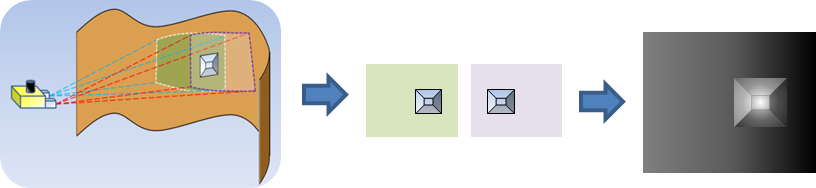
\epsfig{file = pics/2.png, width = 0.9\textwidth}}
   \caption{How we generate disparity maps from images.}
  \label{fig:dispgen}
 \end{figure*}


A number of algorithms currently exist which compare the features of two images in order to determine the distance between the feature and the camera. (Figure~\ref{fig:dispgen}). 
Unfortunately, few of these algorithms are robust enough to handle compressed underwater images of rock walls, due to the poor lighting conditions and very organic, shallow features present.
After exploring several options, the stereo mapping algorithm described by Zitnick and Kanade in ~\cite{stereo:zitKan} was chosen for the current implementation.

The images captured within the cisterns usually represent a landscape with minimal color changes, poor lighting and shallow depressions (in comparison to images with large color or depth contrast).
Rocks bricks, two common features found on the cistern walls, have highly repetitive patterns and colors which produce feature-scarce images.
Most stereo-matching algorithms, including Zitnic and Kanade, rely on defining and matching distinct features.
The algorithm proposed by Zitnick and Kanade uses a scanning, sliding comparison window to build an initial disparity map.
To mitigate the dull landscape, we choose a large initial disparity window with a radius of five pixels.
This decision reduces the level of fine details that can be resolved from the image and adds a smoothing effect to the disparity map, but these drawbacks are acceptable in the given environment.
Instead, a large window gives a more reliable matching between rocks faces because it can encompass more features for each pixel.  

%ZJW read this and make sure you agree
The largest issue we faced in underwater environments was lighting. Most of the water systems we explored were dark (with little light entering the systems through narrow tunnels and openings. The lack of light meant that almost all lighting in the images was from the ROV's onboard lights, requiring the ROV to fly close to the walls in order to illuminate features for the cameras. The ROV has two lights (port and starboard), which resulted in two contrasting lighting conditions for the left and right images. Therefore disparities in lighting between images, and as a result pixel intensities, is a common problem in our images. See Figure~\ref{fig:disparity} for an example of the contrasting lighting. These extreme lighting conditions are not handled well by the Zitnick and Kanade algorithm and potential future solutions to the lighting problem are discussed in greater detail in Section~\ref{subsec:hsl_color_correction}.

Another common challenge in our images were floating dirt particles due to the ROV's positioning thrusters agitating sediment in the water systems. Usually the particles are small enough to be detected and removed from the final disparity map.
%ZJW: say how removed (smoothing?)


\subsubsection{Image Correction}
\label{subsec:image_correction}

In many stereo mapping algorithms, including Zitnick and Kanade, it is assumed that both images are accurate down to the pixel level.
Regrettably, the GoPro cameras used were limited to recording images in the lossy .jpeg format only.
To solve this issue we smoothed and shrunk the high resolution .jpeg images taken by the GoPros to produce smaller left and right images that were comparable at the pixel level.

%ZJW: we should have text that lists the image sizes and then what size they are shrunk to
Image correction starts with a smoothing step  to remove .jpeg artifacts. A simple Gaussian smoothing step was ineffective in this case because it blurred the edges of the rocks or bricks, removing valuable features from an already feature-scarce image. Instead an image smoothing tool was used (Photoshop's "surface smooth") which preserved edges while still blurring similar color regions. Next the shrinking step was performed on the image to further reduce the .jpeg artifacts and trim the size to (x by x). Through experimentation, we discovered that the best image detail to process time ratio was obtained by reducing the images by one sixth.
Shrinking was performed after smoothing to preserve the maximum amount of detail in the image.

\subsubsection{HSL Color Correction}
\label{subsec:hsl_color_correction}
In addition to the general lighting challenges described above, the paired GoPro cameras chosen for data collection lacked the ability to sync exposure times.
The cameras independently calculated the correct exposure for their image only, which resulted in a lack of light intensity matching between left and right images (note the difference in light between the left and right images in Figure ~\ref{fig:disparity}).
A potential solution to this problem lies in using a color comparison function instead of an intensity comparison function ~\cite{stereo:nalGast}.
The solution proposed by Nalpandtidis and Gasteratos suggests converting the images into the HSL color space and looking at only the hue and saturation values.
For our purposes, however, this method failed.  
Many of the surfaces that we imaged were gray in color producing uniform hue and saturation values.
For future experiments, introducing a light with a distinct color, perhaps blue, could prove useful for gray surfaces.  
This blue light would provide definite hue and saturation values that could be compared regardless of exposure times.

\subsubsection{Disparity Mapping}
\label{subsec:disparity_mapping}

Disparity maps were generated using the cooperative, iterative approach described by Zitnick and Kanade ~\cite{stereo:zitKan}.
The basic algorithm is as follows:
\begin{itemize}
\item Find the local support for each pixel at $(x,y)$ and each depth, $d$, by using an image intensity comparison function, $\delta$.
We chose $\delta$ to be a normalized correlation function.

\begin{equation}
L_0(x,y,d) = \delta(I_{Left}(y,x),I_{Right}(y,x+d))
\end{equation}

\item Copy the values from the 3D array $L_0$ into a new 3D array, $L_n$.

\item Assume that $\Phi(x,y,d)$ is the 3D support region around the pixel $(x,y)$, and suppose

\begin{equation}
S_n(x,y,d) = \sum_{(x',y',d') \in \Phi} L_n (x+x', y+y', d+d')
\end{equation}

Furthermore, assume that $\Psi(x,y,d)$ is the set of all pixels that map to $(x,y)$ in the left image and $(x+d,y)$ in the right image. 
Let $\alpha$ be a constant that controls how quickly the values in $L_n(x,y,d)$ will converge. Then, iterate through the values in $L_n$ updating each value using
 
\begin{align}
L_{n+1}(x,y,d) &= \\ 
L_n(x,y,d)\left(\frac{S_n(x,y,d)}{\sum\limits_{(x'',y'',d'') \in \Psi(x,y,d)} S_n(x'',y'',d'')} \right)^\alpha 
\end{align}

\item To build the final disparity map, loop through each pixel position $(x,y)$ and award the depth value $d$ with the highest weight from $L_n(x,y,d)$ as the final value.
If the best weight for all depths for a certain pixel $(x,y)$ is below a predefined threshold, assume the pixel was occluded.
\end{itemize}

%\subsubsection{Post Disparity Generation Correction}
%\label{subsec:post_zitcan_correction}

%All of the disparity maps generated by the Zitnick and Kanade algorithm had slight errors around the edges.  
%Patches of the image would either be unreasonably close to the camera or flat against the background.  
%These images had to be corrected before they could be mapped to vertices.  




\subsection{Calibration}
\label{subsec:calibration}

An important step in any meaningful disparity mapping is calibration.
This is the creat
Pictures of a patterned surface were taken at a number of measured distances from that surface.
Those images were then disparity mapped, and the average disparity at the center of the picture was used as the disparity data point for that physical depth.
Using this set of points we were able to create a linear mapping between disparity and depth.

%ZJW: conclusion about calibration?

%ZJW: Need a concluding paragraph about disparity map generation - Also should you say something about smoothing out spurrious data?
Once a disparity map has been generated, it can be used as depth values to displace the general geometry created from the sonar data. See Figure~\ref{fig:disparity} illustrates a disparity map generated using our implementation.


\subsection{Projective Texturing}
\label{subsec:projectiveTexturing}

%ZJW: need to motivate projective texturing - please read what I wrote and edit as desired
\noindent In order to add fine details to the general mesh created from sonar data, $M_s$, we need to map the location of the disparity map data onto the global coordinates of the general mesh. Ideally, real localization would be used to correspond the coordinates of the general mesh and the displacements (i.e. solve the ROV's location in the mapped model when the images were captured).  With our current hardware, ROV localization is only computed for fixed scans and we do not know where the ROV is with respect to the map for every image acquired. Future work includes using additional hardware such as a smart tether to assist in localization, but for our preliminary results, we use projective texturing with a user's input to place color and disparity data correctly. In general, the ROV captures an image of an organic feature in a cistern, and our implementation allows the user to position a projector which casts the image from the same relative position onto the general mesh for displacement (Figure~\ref{fig:dispgen}). Projective texturing is  utilized because of its ability to properly simulate an ROV as a point particle with the ROV's view frustum modeled as six implicit plane equations (i.e. modeling the camera field of view). Our implementation allows the projection of multiple textures and disparities, building a more detailed and colored model as more images and disparities are placed and added to the original mesh.

The combination of projective texturing and stereoscopic imaging enables the ability to selectively displace vertices according to the color of a texture-mapped disparity map that is projected onto a surface. These vertices are displaced along the vector leading from their original 3D position in the mesh to the position of the projector, re-applying the geometry captured within the cistern to the model.  For our implementation uses, OpenGL and OpenGL Shading Language (GLSL) graphics libraries to aid in projective texturing, the latter being used to create shaders - small programs run per-vertex directly on the GPU. The shaders are programmed to selectively alter rendered vertex information, such as position (vertex shader) and color (fragment shader). 

A projector is simulated by establishing plane equations for a view frustum based on the position and orientation of the ROV when the projected images were captured in a cistern. We define $J = \{j_{1},\dots,j_{N}\}$ to be the set of projectors casting textures onto the gross surface reconstruction. Each projector, $j_{n} = ((j_{n_{x}}^{pos},j_{n_{y}}^{pos},j_{n_{z}}^{pos}), \langle j_{n_{x}}^{look},j_{n_{y}}^{look},j_{n_{z}}^{look}\rangle)$, is uniquely defined by its position in 3D space, and a look vector orthonormal to the projector's viewport (Figure~\ref{fig:frustum}). All projectors have a pre-calibrated Field Of View (FOV) mimicking the compound FOV produced by the GoPro camera and waterproof housing lenses. The ROV is not equipped with roll thrusters, allowing us to ignore the possibility of a tilted camera frustum (i.e. the projector's right facing vector will always lie in the horizontal plane). Implicit plane equations modeling the projector view frustums in the form $Ax + By + Cz + D = 0$ are resolved using the clip space approach~\cite{vfc}, where $\langle A, B, C\rangle$ is the plane's normal vector and  $(x, y, z)$ is a point on the plane. In this approach, plane equations are computed in homogenous space using the composite $4x4$ modelview projection matrix of the projector, $\lbrack \chi \rbrack$.

\begin{align}
\nonumber %Left plane
&\lbrack A \hspace{3pt} B \hspace{3pt} C \hspace{3pt} D \rbrack^\mathrm{T}_{Left} \hspace{-15pt} &= \hspace{10pt}&\lbrack \chi_{11} \cdots \chi_{41} \rbrack^\mathrm{T} + \lbrack \chi_{14} \cdots \chi_{44} \rbrack^\mathrm{T}
\\
\nonumber %Right plane
&\lbrack A \hspace{3pt} B \hspace{3pt} C \hspace{3pt} D \rbrack^\mathrm{T}_{Right} \hspace{-15pt} &= -&\lbrack \chi_{11} \cdots \chi_{41} \rbrack^\mathrm{T} + \lbrack \chi_{14} \cdots \chi_{44} \rbrack^\mathrm{T}
\\
\nonumber %Top plane
&\lbrack A \hspace{3pt} B \hspace{3pt} C \hspace{3pt} D \rbrack^\mathrm{T}_{Top} \hspace{-15pt} &= \hspace{10pt}&\lbrack \chi_{12} \cdots \chi_{42} \rbrack^\mathrm{T} + \lbrack \chi_{14} \cdots \chi_{44} \rbrack^\mathrm{T}
\\
\nonumber %Bottom plane
&\lbrack A \hspace{3pt} B \hspace{3pt} C \hspace{3pt} D \rbrack^\mathrm{T}_{Bot} \hspace{-15pt} &= -&\lbrack \chi_{12} \cdots \chi_{42} \rbrack^\mathrm{T} + \lbrack \chi_{14} \cdots \chi_{44} \rbrack^\mathrm{T}
\\
\nonumber %Near plane
&\lbrack A \hspace{3pt} B \hspace{3pt} C \hspace{3pt} D \rbrack^\mathrm{T}_{Near} \hspace{-15pt} &= \hspace{10pt}&\lbrack \chi_{13} \cdots \chi_{43} \rbrack^\mathrm{T} + \lbrack \chi_{14} \cdots \chi_{44} \rbrack^\mathrm{T}
\\
\nonumber %Far plane
&\lbrack A \hspace{3pt} B \hspace{3pt} C \hspace{3pt} D \rbrack^\mathrm{T}_{Far} \hspace{-15pt} &= -&\lbrack \chi_{13} \cdots \chi_{43} \rbrack^\mathrm{T} + \lbrack \chi_{14} \cdots \chi_{44} \rbrack^\mathrm{T}
\\
\end{align}

\begin{figure}[!h]
   \vspace{-0.2cm}
   \centering{
      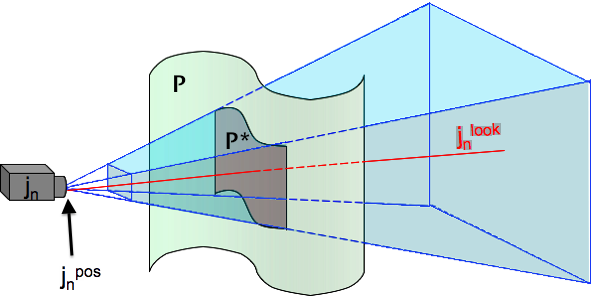
\epsfig{file = pics/frustum.png, width = 7cm}}
   \caption{Frustum and viewport.}
  \label{fig:frustum}
 \end{figure}

In order to optimize the projection step and only displace and color vertices in the current view, for each projector, all faces in the mesh are passed through a view frustum culling filter in order to produce a list of faces contained within the current frustum. We define $P = \{p_{1},\dots,p_{M}\}$ to be the set of vertices of the general mesh, $M_s$. Each vertex, $p_{n} =  (p_{m_{x}},p_{m_{y}},p_{m_{z}})$, is defined by its position in 3D space. Additionally, we define $F = \{f_{1},\dots,f_{Q}\}$ as the set of faces in the mesh, $M_s$. Each face, $f_{q} = (p_{\alpha}, p_{\beta}, p_{\gamma})$, is comprised of three vertices. We begin with a preliminary culling which discards faces if their bounding sphere is outside of the projector's view frustum. Since frustum planes are modeled implicitly with normal vectors pointing into the frustum, if the signed distance from the face's center to the frustum plane, $\delta_{center}$, is less than the negative of the face's bounding sphere's radius, then the face's bounding sphere is entirely outside of the view frustum. In this case the face is immediately culled. $\delta_{center}$ is computed as follows,
%
\begin{equation}
\delta_{center} = \frac{Ax + By + Cz + D}{3 \begin{Vmatrix} \langle A, B, C \rangle \end{Vmatrix}},
\end{equation}

where
\begin{equation}
(x, y, z) = \left(\sum\limits_{\forall p_{m} \in f_{q}} p_{m_{x}}, \sum\limits_{\forall p_{m} \in f_{q}} p_{m_{y}}, \sum\limits_{\forall p_{m} \in f_{q}} p_{m_{z}}\right)
\end{equation}

Once faces are passed through the preliminary culling filter, a more precise culling is executed in order to remove the small number of faces that lie entirely outside of the frustum, but whose bounding spheres intersect the frustum.  To accomplish this, the signed distances from each vertex in the face to the frustum plane, $\delta_{\alpha}$, $\delta_{\beta}$, and $\delta_{\gamma}$, are individually computed. If $\delta_{\alpha}$, $\delta_{\beta}$, and $\delta_{\gamma}$ are all less than zero, the face is culled. $\delta_{\alpha}$, $\delta_{\beta}$, and $\delta_{\gamma}$ are computed as follows,
%ZJW: this section is slightly detailed - but since we may end up submitting to a more general conference (not graphics specific, we can leave in for now unless we need space later, in which case we can compress this section a good deal

\begin{equation}
\delta_{\alpha, \beta, \gamma} = \frac{Ax + By + Cz + D}{\begin{Vmatrix} \langle A, B, C \rangle \end{Vmatrix}},
\end{equation}

where
\begin{align}
\nonumber
(x, y, z)_{\alpha} &= (p_{\alpha_{x}}, p_{\alpha_{y}}, p_{\alpha_{z}})\\
\nonumber
(x, y, z)_{\beta} &= (p_{\beta_{x}}, p_{\beta_{y}}, p_{\beta_{z}})\\
(x, y, z)_{\gamma} &= (p_{\gamma_{x}}, p_{\gamma_{y}}, p_{\gamma_{z}})
\end{align}


With faces lying outside of the projector view frustums culled, the vertices in the remaining faces are added to a trimmed set, $P^{*}\subset P$, whose members are sent to the vertex and fragment shaders (i.e. to the GPU) to be displaced and textured in accordance with the generated disparity map and camera image, respectively (Figure~\ref{fig:frustum}). $P$ is also sent to the GPU so that the portions of the mesh that are not displaced or textured are still rendered.

The implemented projective texturing method naturally produces a second projection facing in the direction negative to $j_{n}^{look}$. To remove the unwanted projections, a simple check was added to the vertex shader which ensures that the texture mapped vertex position has a positive $q$ component.

\subsection{Per-Vertex Displacement Computations}

A GLSL vertex and fragment shader are used to displace and texture vertices. The vertex shader recieves $P$ and $P^{*}$, as well as a modelview projection matrix for the camera and each projector, projector positions, texture primitives for the disparity maps, an offset and scale value for displacement magnitudes, and normal vectors used for lighting computations from the OpenGL program. The vertex shader displaces vertices one at a time in accordance with the color of the texture-mapped disparity map coordinates. Vertices belonging to $P^{*}$ are updated and sent to the fragment shader for diffuse shading computations.

The fragment shader recieves $P$ and $P^{*}$, as well as the camera image texture primitives and the revised normal vectors of the vertices in $P^{*}$. The fragment shader maps the camera images onto the vertices in the frustum of each projector. Again, vertices lying in the frustum of two or more projectors have their colors blended. Once an RGB color value has been computed for the vertex, diffuse shading is added to the model.

\subsubsection{Vertex Displacement}

Vertices belonging to $P^{*}$ are displaced along the vector $\vec{b} = j_{n} - p_{m}$ a distance proportional to the magnitude of the RGB color value, $\vec{C} = \langle C_{r}, C_{b}, C_{g} \rangle$, of the disparity map at the corresponding texture-mapped coordinates, $t_m$. Since the modelview projection matrix of each projector is accessible from the vertex shader, the texture-mapped coordinates of $p_m$, and thus, $\vec{C}$ can be calculated per-vertex.

\begin{align}
t_{m} &= p_{m}\lbrack MVP \rbrack _{j_{n}} \\
\vec{C} &= \langle t_{m\_red}, t_{m\_blue}, t_{m\_green} \rangle
\end{align}

Vertex displacement then proceeds as follows:

\begin{equation}
p_{m}' = \left \{ 
\begin{array}{ll}
p_{m} + \vec{b} (\begin{Vmatrix}\vec{C}\end{Vmatrix} S + O) & \text{if} \quad p_{m} \in P^{*}\\
p_{m} & \text{otherwise}
\end{array},\right.
\label{eq:displace}
\end{equation}

where $p_{m}'$ is the displaced vertex position and $S$ and $O$ are a scale and offset factor. $S$ grants the ability to fit a function to the displacement distance.$O$ is generally negative, ensuring that vertices belonging to $P^{*}$ are both pushed and pulled from the model surface rather than only being pulled towards the projector. In the current version of the software, both $S$ and $O$ are user-controlled. However, the world space coordinates of $M_s$ are computed such that one unit in world space is equal to one meter in the cistern, so a true value for $S$ and $O$ can be calculated through further calibration.
 
 \subsubsection{Projection Blending}

%Feel free to remove/edit/use for inspiration
The existence of multiple projections in the virtual cistern requires the ability to artfully and accurately overlap those projections.
A projection consists of both a texture and a disparity map.
Each single projection is just as likely of being the ground truth data for a vertex as any other projection that is applied to that vertex. 
Thus, each projection that is applied to a vertex has equal weight upon that vertex's final color and position.
Let us assume $J_1$ is the set of all projectors casting a disparity value onto this vertex and let $B = \{j \in J_1 : (j - p_m)\}$. 
Then expanding on equation ~\ref{eq:displace} for q overlapping projections,

\begin{equation}
p_{m}' = \left \{ 
\begin{array}{ll}
p_{m} + \sum\limits_{\vec{b} \in B} \frac{(\vec{b} \begin{Vmatrix}\vec{C}\end{Vmatrix} S + O)}{q} & \text{if} \quad p_{m} \in P^{*}\\
p_{m} & \text{otherwise}
\end{array},\right.
\label{eq:displaceBlend}
\end{equation}

Similarly, to determine the final color of the vertex, let $\vec{C_t}$ be the final color of a vertex and let $C_p$ be the set of all colors projected onto that vertex. 
\begin{equation}
\vec{C_t} = \sum\limits_{\vec{c} \in C_p} \frac{\vec{c}}{q} 
\label{eq:colorBlend}
\end{equation}

There are other, more complex, methods we could use to weight certain projections higher than others, for example by considering distance to the wall and viewing angle, but this simple averaging scheme has worked in practice. 

\subsubsection{Post-Displacement Lighting Recalculation}

The displacement of vertices necessitates a normal vector recalcuation within the vertex shader. Unfortunately, neighboring vertex information is not available in the vertex shader, making true Phong shading calculations difficult. Instead an approximation is used for the new normals which does not require information regarding neighboring vertices.

Assuming vertices in a close vicinity to each other are displaced roughly the same amount, as a vertex is displaced towards a projector, the true normal vectors of the surrounding faces begin to grow towards the displacement vector. While this assumption is imperfect near edges and crevices present in the disparity maps, it has been found to work well in practice. 
%ZJW re-write this -- and do you have an image of just a grey shaded mesh with new normals?
Given this information, we require a lighting calculation such that normals are equal to the negative of the displacement vector at an infinite displacement from the projector, normals are equal to their original values if vertices are not displaced, and normals grow towards the displacement vector as vertices are displaced towards the projector. Due to these constraints, the approximate normal computation for diffuse shading on displaced vertices is as follows:

\begin{equation}
   n_m^* = \left \{ \begin{array}{ll}
      n_m + \left(\hat{d} \exp\left(\begin{Vmatrix}\vec{d}\end{Vmatrix}\right) - \hat{d}\right) & \text{if} \quad \vec{b} \cdot \vec{d} > 0 \\
      n_m + \left(\hat{d} \exp\left(-\begin{Vmatrix}\vec{d}\end{Vmatrix}\right) -   \hat{d}\right) & \text{otherwise}
   \end{array},\right.
\label{eq:lighting}
\end{equation}


where $n_m$ is the vertex's normal, $n_m^*$ is the updated normal vector, and $\vec{d} = \begin{Vmatrix}\vec{C}\end{Vmatrix} S + O$ is the displacement vector from~\eqref{eq:displace}.

Couple more sentences of explanation here...

\section{\uppercase{Results}}
\label{sec:results}

To demonstrate our complete cistern mapping system we deployed our ROV in a rock-walled well in a courtyard in the church, Convento dei Cappuccini, in Council of Carini (near Palermo, Sicily).
This cylindrical shaped well was built with rocky walls.  Using the sonar data acquired during the deployment a rough 3D model shown in Figure~\ref{fig:wellNoFine} was constructed.  This model is a good representation of the gross shape of the well, but lacks the geometric details of the rocky walls.  During this deployment, the GoPro camera were also mounted on the ROV and stereo pairs were captured for use in generating disparity maps.

Our implementation of the Zitnick and Kanade algorithm was shown to perform well against the Univerisity of Tsukuba's Multiview Image Database ~\cite{stereo:zitKan}, and with the appropriate image filtering and parameter settings (described above) it performed similarly well with rocky underwater cistern images.
One such output image is show in Figure~\ref{fig:disparity}.
%ZJW, I think we should include another figure like this, to show at least two different disparities...  if there is enough room
This image was generated using an initial support region of size (11, 11, 5), and then an iterative local support region of size (13,13,5).
Note that the left and right images demonstrate a difference in lighting.
%ZJW: is there anything else we can say about your implementation or parameter setting to differentiate this work from just a generic re-implementation?

\begin{figure}[!h]
	\centering
		\subfigure[Left camera image]{\label{left}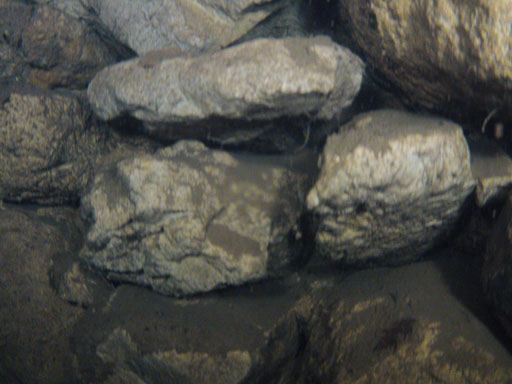
\epsfig{file = pics/372L.jpg, width = 3cm}}
		\quad %space between images
		\subfigure[Right camera image]{\label{right}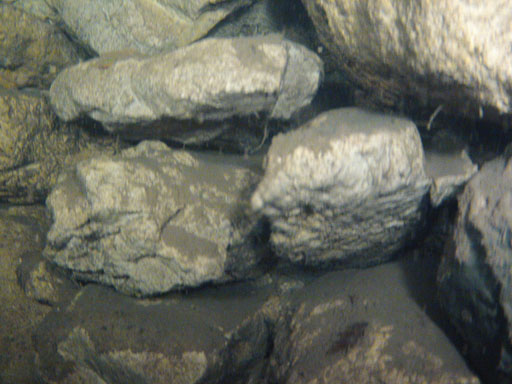
\epsfig{file = pics/372R.jpg, width = 3cm}}\\%new line
		\medskip
		\subfigure[Generated Disparity Map]{\label{disparitymap}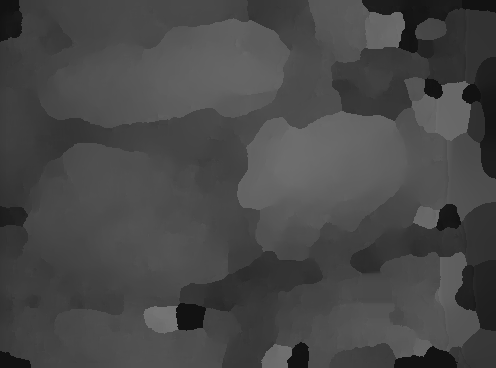
\epsfig{file = pics/372disp.png, width = 5cm}}
		\caption{An example disparity map generated with initial local support region of (13,13,5), and an iterative support region of (11,11,5).}
		\label{fig:disparity}
\end{figure}


\begin{figure}[!h]
	\centering
		\subfigure[Well Top View]{\label{left}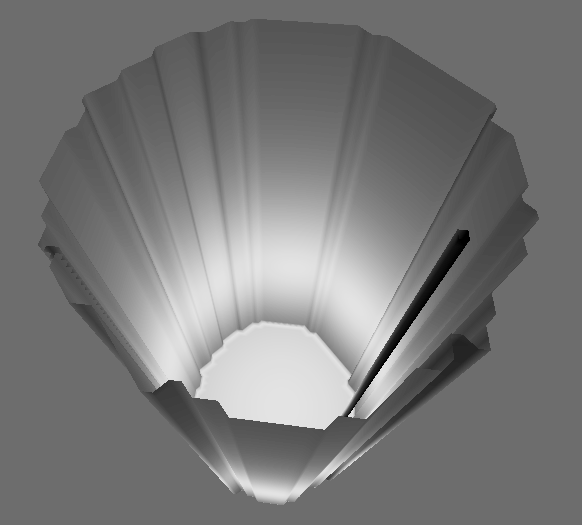
\epsfig{file = pics/blankWell3.png, width = 3.5cm}}
		\quad %space between images
		\subfigure[Well Side View]{\label{right}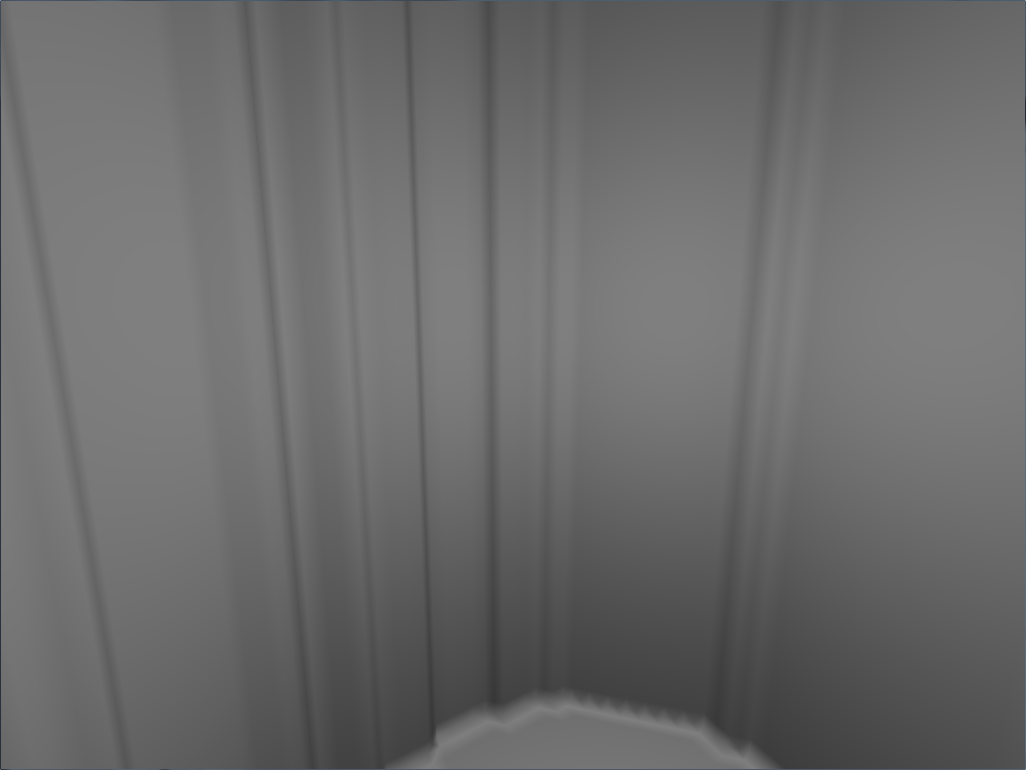
\epsfig{file = pics/blankWell2.png, width = 3.5cm}}\\%new line

		\caption{Views of Plain Well Geometry}
		\label{fig:wellNoFine}
\end{figure}

\begin{figure}[!h]
	\centering
		\subfigure[Well Photo]{\label{right}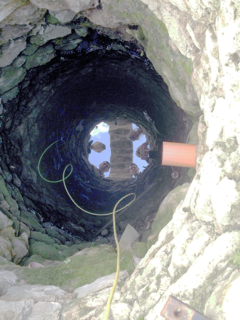
\epsfig{file = pics/wellPhoto, width = 3.5cm}}\\%new line

		\caption{ A photograph of the walls of the well.}
		\label{fig:wellPhoto}
\end{figure}

Using the geometry from the general mesh constructed from the sonar data, we used virtual point projectors to display the rock images and disparity maps as they were originally captured at that location.  
The disparity maps were further used to deform the well geometry as shown in Figure ~\ref{fig:result2} (b).

\begin{figure}[!h]
	\centering
		\subfigure[Projected Images]{\label{left}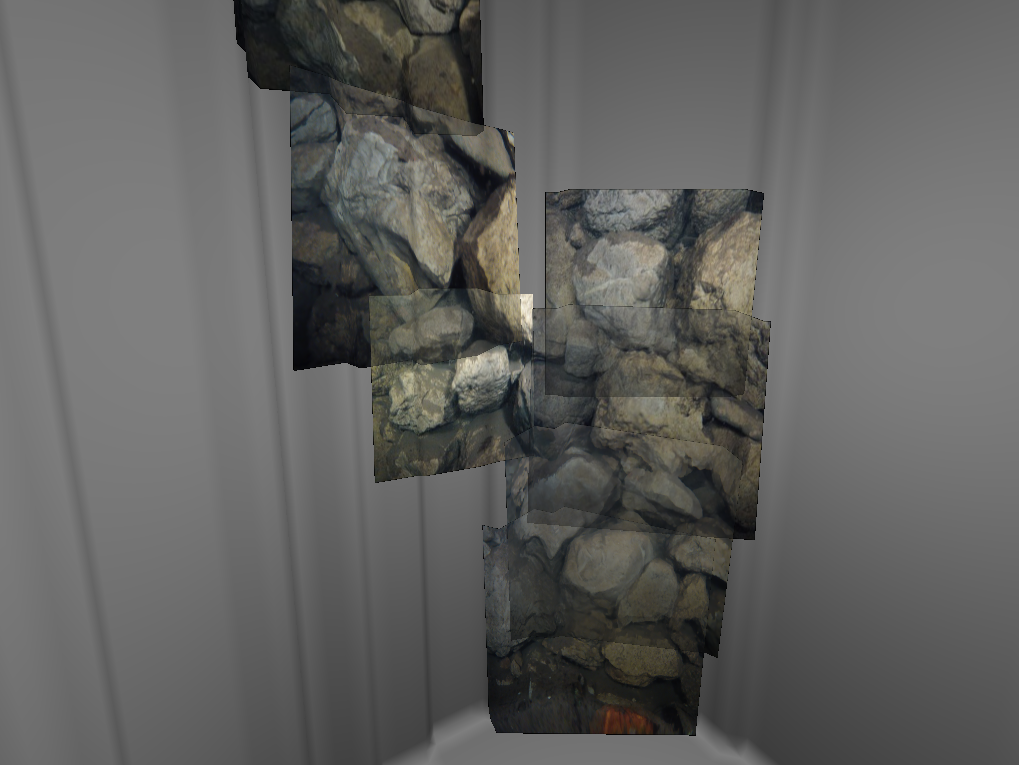
\epsfig{file = pics/noDisparity.png, width = 6.5cm}}\\
		\quad %space between images
			\subfigure[Projected Disparity maps]{\label{left}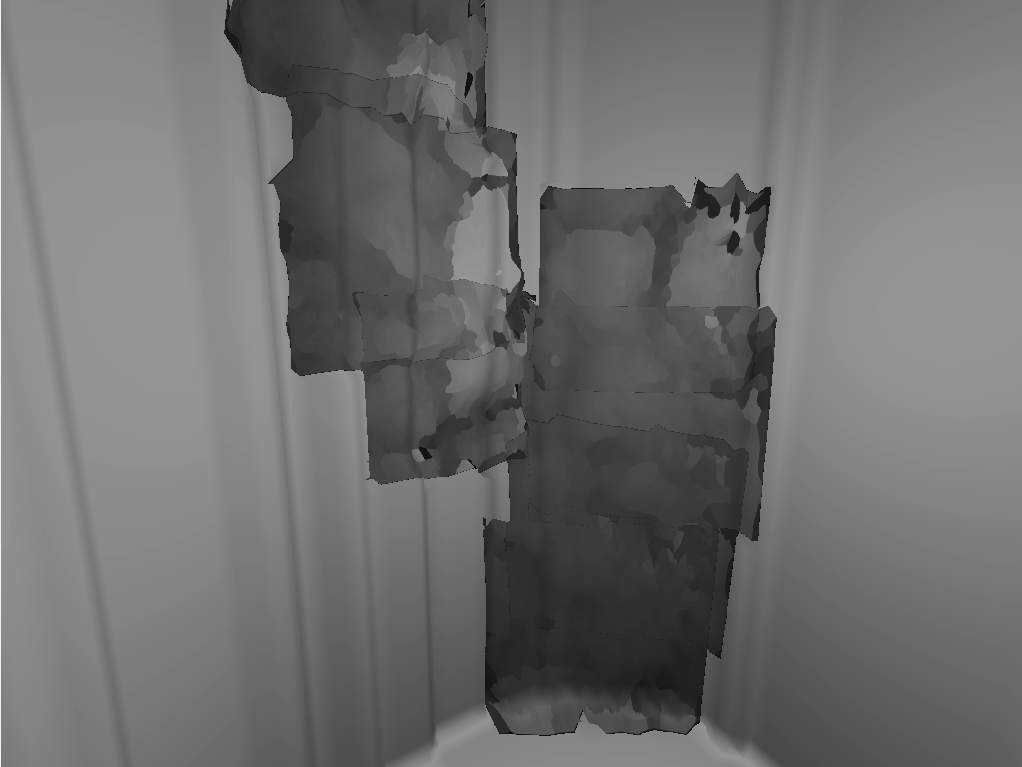
\epsfig{file = pics/mapsDisparity.png, width = 6.5cm}}\\		
	
		\caption{A set of images and disparity maps reprojected as they were captured inside the well. This well sits in a courtyard in a church, Convento dei Cappuccini, in Council of Carini (near Palermo, Sicily)}
		\label{fig:result2}
\end{figure}

%  The disparity maps calculated at each of those points were then applied to deform the well geometry (Figure ~\ref{fig:result4}).
%
%\begin{figure}[!h]
%	\centering
%		\subfigure[Images on Wireframe]{\label{right}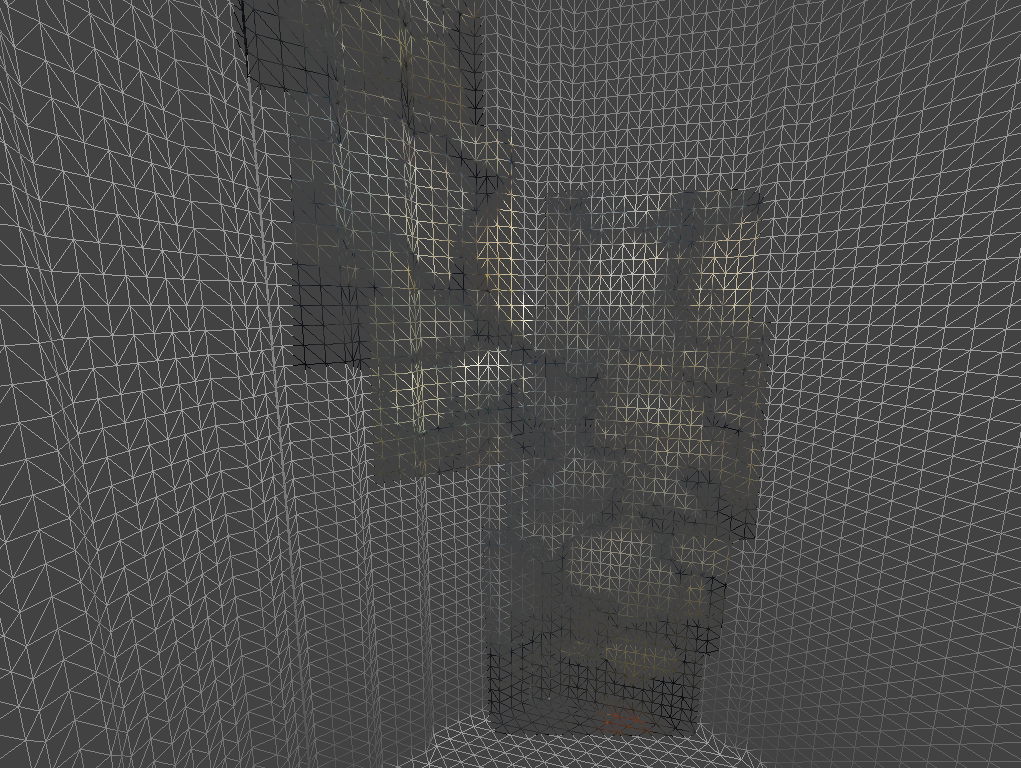
\epsfig{file = pics/noDisparityWire.png, width = 3.5cm}}\\%new line
%		\quad %space between images
%		\subfigure[Wireframe Disparity Maps]{\label{right}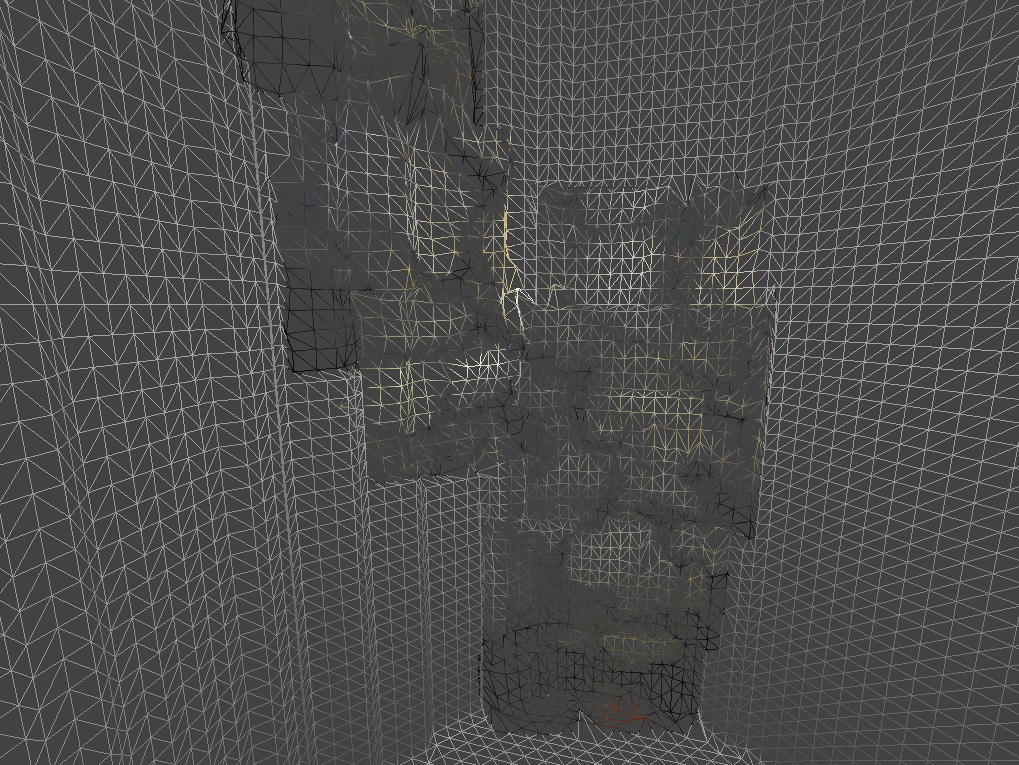
\epsfig{file = pics/disparityWire.png, width = 3.5cm}}\\%new line
%		\caption{Well Deformed by Disparity Maps}
%		\label{fig:result3}
%\end{figure}

Finally, the disparity maps combined with the surface images were mapped into the well geometry to produce the detailed mesh in Figures~\ref{fig:result4} \&~\ref{fig:resultFull}. In our current implementation all textures are stored on the GPU, which limits the number we can currently display to X. Future work will include methods to cycle through textures.
%he only factor that is keeping us from filling the well with textures is the Glew texture limit. ???
%ZJW: really???  we need a way around that - Once you've displaced and colored vertices can't you release a texture and cycle through more? - the above sounds fairly weak....

%need to figure out how to do a gradient fade between wireframe and real images
\begin{figure}[!h]
	\centering
%		\subfigure[Well Wide Shot]{\label{left}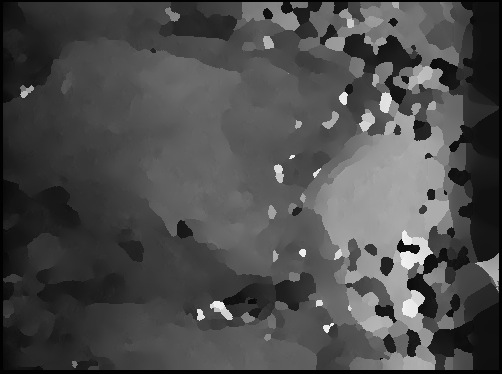
\epsfig{file = pics/disparity.png, width = 3.5cm}}
%		\quad %space between images
%		\subfigure[Rocks Closeup]{\label{right}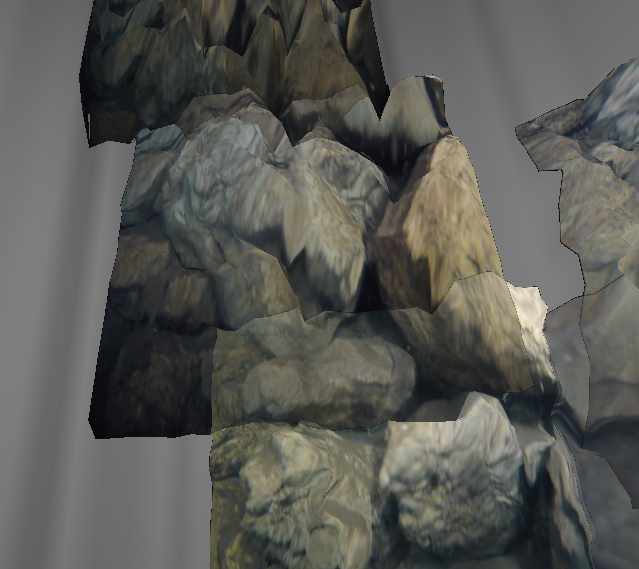
\epsfig{file = pics/mappedWell1.png, width = 3.5cm}}\\%new line
%		\medskip
		\subfigure[Rocks Closeup Wireframe]{\label{center}\epsfig{file = pics/closeFinal4.png, width = 7cm}}
		\caption{Fully Mapped Well}
		\label{fig:result4}
\end{figure}

\begin{figure*}[!ht]
   \vspace{-0.2cm}
   \centering{
      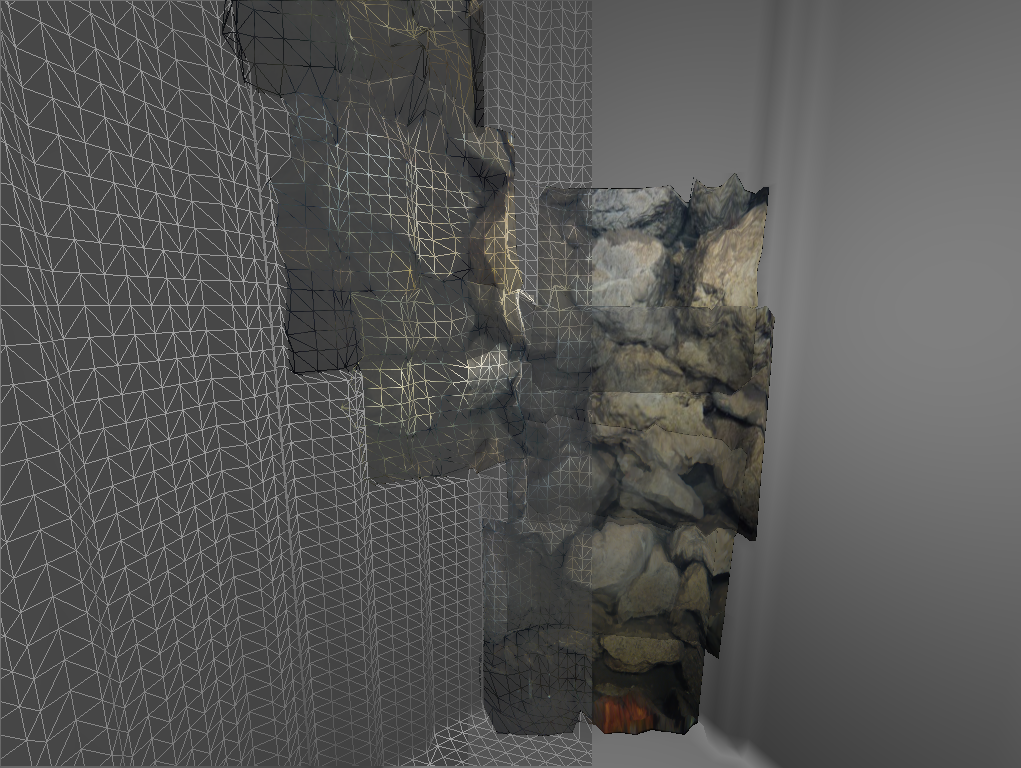
\epsfig{file = pics/halfDisparity.png, width = .9\textwidth}}
   \caption{Detailed view of multiple displacement maps and color data mapped onto part of the general mesh.  The geometric details added by the disparity maps creates a much better geometric model of the walls of the well.}
  \label{fig:resultFull}
 \end{figure*}

%\begin{figure*}[!ht]
%   \vspace{-0.2cm}
%   \centering{
%      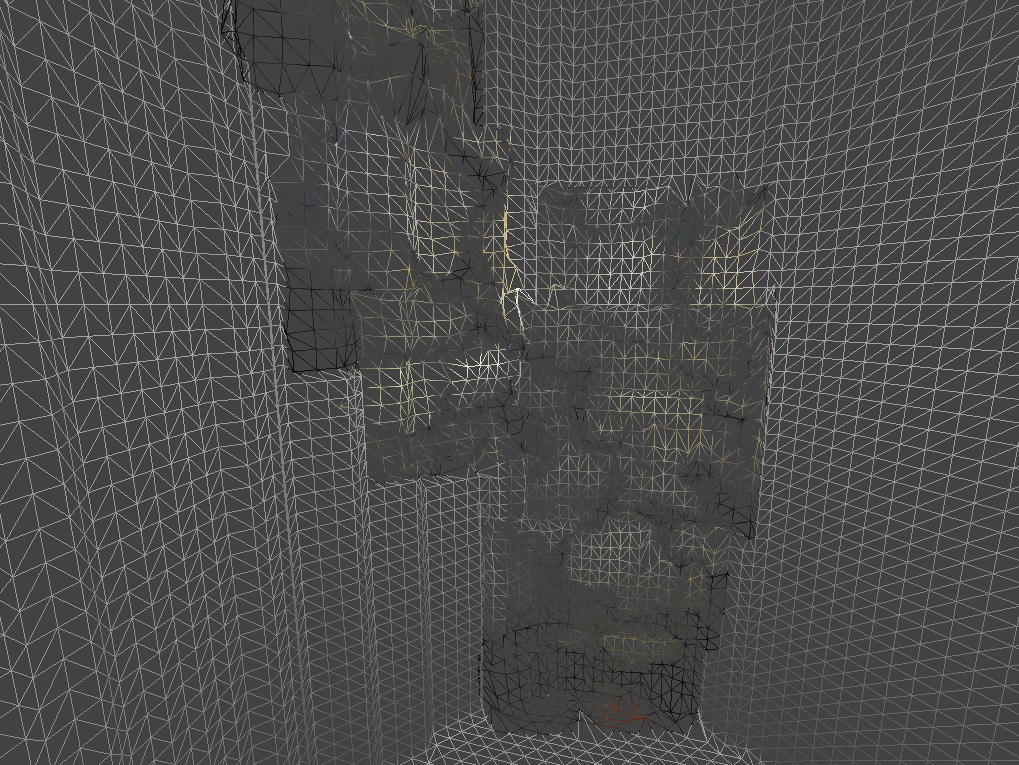
\epsfig{file = pics/disparityWire.png, width = .9\textwidth}}
%   \caption{Full Displaced Well, Wireframe}
%  \label{fig:resultFullWire}
% \end{figure*}

\section{\uppercase{Conclusion and Future Work}}
\label{sec:conclusion}

\noindent 
This paper presents a novel way to add geometric details to maps created to represent underwater environments. A general model is acquired from sonar data and mapping~\cite{ICEX11,McVicker,McVicker2}, and we present the addition of fine level details using stereo image data.  This work is motivated by the desire to better map underwater caverns and cisterns using robotic tools.  We have presented our methodology and hardware for data acquisition, disparity map generation, and incorporation of that disparity data via projective texturing displacements.  We have shown results of a partial reconstruction of a well in Carini, Sicily.

In this preliminary work, we have discovered many of the key factors for obtaining more complete models and details.  Future enhancements include: the creation of more detailed disparity maps, inclusion of color lighting, inclusion of smart tether for better localization, enhancements to memory management to process more textures and disparity maps at once.
For example, more detailed disparity maps could be achieved by upgrading the cameras and the lights on the robot.
GoPro cameras were a simple, cost-effective, solution to acquire underwater stereo images.
The quality of the captured images, however, could be greatly increased with more professional hardware.
With better cameras the output images would not need to be processed down to remove jpeg compression artifacts, which would allow much larger disparity images.  
Similarly, with better cameras there would be no need to compensate for different exposure times between images, and images could be captured synchronously.
Alternatively, better lighting, including blue lights, would allow pixel values to be compared in the HSL color space.
Such lighting additions would reduce the need for a different camera setup.

Data collection in future deployments will be performed during a dry spell, as flowing rainwater dirtied the water and reduced image quality. Since the clearest pictures were taken before the ROV had uplifted sediment from the cistern floor by landing, the ROV will capture all images of the cistern wall before landing to record sonar scans. Additionally, none of the image data sets from the previous expedition captured the entirety of the walls in a cistern. In subsequent deployments, the entire wall of each cistern will be captured.

With regards to shader calculations, a second vertex shader could be implemented in order to compute Phong shading on the displaced vertex positions. Additionally, we would like to explore algorithms from texture synthesis and apply learning to a small subset of disparity images in order to generalize the small detailed geometry without having to acquire disparity maps of the entire wall.

In the future it would be interesting to explore the possibility of integrating this algorithm with a SLAM algorithm and more computing power to allow a robot to autonomously image each surface of a cistern. 
Unfortunately, that would require a far more complex setup that what we had available at the time of writing.

%ZJW: Please add some suggestion for actual data collection methods as well - re: lighting, positioning ROV, etc.

\bibliographystyle{apalike}

\bibliography{stereo}

\end{document}

